\documentclass[11pt]{article}
\usepackage{graphicx} % Required for inserting images
\usepackage{amsmath, amssymb, graphicx, enumerate}
\usepackage[margin=0.5in]{geometry}
\graphicspath{{./}}



\title{3.1 Extrema on an interval}
\author{Juan J. Moreno Santos}
\date{October 2023}

\begin{document}

\maketitle

\section{Value of derivate (if it exists) at each indicated extremum}
2.\[f(x)=\cos\frac{\pi}{2}\]
\[f'(x)=\frac{(2x)(x^2+4)-(x^2)(2x)}{(x^2+4)^2}=\frac{8x}{(x^2+4)^2}\therefore f'(0)=0\]

\vspace{1cm}
\noindent
4.\[f(x)=-3x\,\,\sqrt[]{x+1}\]
\[f'(x)=-3x\left(\frac{1}{2}{(x+1)}^{-1/2}\right)+\sqrt[]{x+1}(-3)\]

\noindent
\section{Approximate the critical numbers of the function shown in the graph. Determine whether the function has a relative maximum, a relative minimum, an absolute maximum, an absolute minimum, or none of these at each critical number on the interval shown}
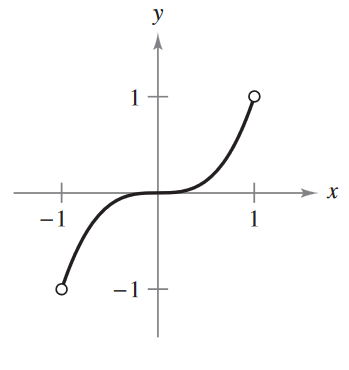
\includegraphics{8.png}\\
8. $x=0$ is a critical number.\ There is no minima or maxima at x=0.

\noindent
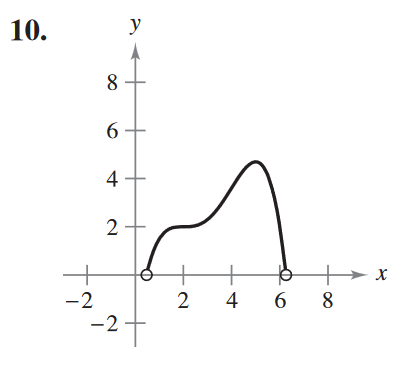
\includegraphics{10.png}\\
10. $x=2, 5$ are critical numbers.\ There is an absolute and relative maximum at $x=5$, and no minima or maxima at $x=2$

\noindent
\section{Find any critical numbers of the function.}
12.\[g(x)=x^4-4x^2\]
\[g'(x)=4x^3-8x=4x(x^2-2)\]
$x=0, 2$ are critical numbers.

\vspace{1cm}
\noindent
14.\[f(x)=\frac{4x}{x^2+1}\]
\[f'(x)=\frac{(4x)(x^2+1)-(4x)(2x)}{(x^2+1)^2}=\frac{4(1-x^2)}{(x^2+1)^2}\]
$x=\pm 1$ are critical numbers.

\vspace{1cm}
16.\begin{eqnarray}
    \setcounter{equation}{1}
    f(\theta)&=2\sec(\theta)+\tan(\theta), \,\,\,0<\theta<2\pi\\
    f'(\theta)&=2\sec\theta\tan\theta+\sec^2\theta\\
    &=\sec\theta(2\tan\theta+\sec\theta)\\
    &=\sec\theta\left(2\left(\frac{\sin\theta}{\cos\theta}\right)+\frac{1}{\cos\theta}\right)\\
    &=\sec^2\theta(2\sin\theta+1)
\end{eqnarray}
$\theta=\frac{7\pi}{6}, \frac{11\pi}{6}$ are critical numbers in $(0, 2\pi)$.

\section{Locate the absolute extrema of the function on the closed interval.}
\noindent
18.\begin{eqnarray}
    \setcounter{equation}{1}
    f(x)=\frac{2x+5}{3}, [0, 5]\\
    f'(x)=\frac{2}{3}\therefore\text{there are no critical numbers}
\end{eqnarray}
$(0, \frac{5}{3})$ is the left endpoint and minimum, and $(5, 5)$ the right endpoint and maximum.

\vspace{1cm}
\noindent
22.\begin{eqnarray}
    \setcounter{equation}{1}
    f(x)&=x^3-12x, \,\,\,[0, 4]\\
    f'(x)&=3x^2-12=3(x^2-4)
\end{eqnarray}
$(0, 0)$ is the left endpoint, $(2, -16)$ is a critical number and the minimum, and $(4, 16)$ the right endpoint and the maximum.

\vspace{1cm}
\noindent
24.\begin{eqnarray}
    \setcounter{equation}{1}
    g(x)&=\sqrt[3]{x}, \,\,\,[-1, 1]\\
    g'(x)&=\frac{1}{3x^{2/3}}
\end{eqnarray}
$(-1, 1)$ is the left endpoint and minimum, $(0, 0)$ is a critical number, and $(1, 1)$ is the right endpoint and maximum.

\vspace{1cm}
\noindent
26.\begin{eqnarray}
    \setcounter{equation}{1}
    f(x)&=\frac{2x}{x^2+1}, \,\,\,[-2, 2]\\
    f'(x)&=\frac{(2)(x^2+1)-(2x)(2x)}{(x^2+1)^2}
    &=\frac{2-2x^2}{(x^2+1)^2}\\
    &=\frac{2(1-x^2)}{(x^2+1)^2}
\end{eqnarray}
$(-2, -\frac{4}{5})$ is the left endpoint, $(-1, -1)$ is the minimum and a critical number, $(1, 1)$ is the maximum and a critical number, and $(2, \frac{4}{5})$ is the right endpoint.

\vspace{1cm}
\noindent
32.\[\lfloor2-x\rfloor,\,\,\, [-2, 2]\]\\
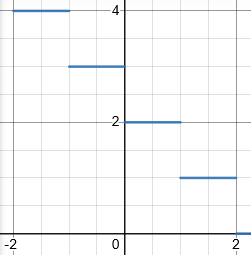
\includegraphics{32.png}\\
Analyzing the graph, the maximum $h$ value is $4$ at $x=-2$, and the minimum is $0$ for $1<x\leq2$.

\vspace{1cm}
\noindent
36.\begin{eqnarray}
    \setcounter{equation}{1}
    y=\tan(\frac{\pi x}{8}),\,\,\,[0, 2]\\
    y'=\frac{\pi}{8}\sec^2(\frac{\pi x}{8})\therefore y'\neq0
\end{eqnarray}
$(0, 0)$ is the minimum and left endpoint, and $(2, 1)$ is the maximum and right endpoint.

\section{Locate the absolute extrema of the function (if any exist) over each interval.}
38. $f(x)=5-x$
\begin{enumerate}[(a)]
    \item $[0, 2]$
    \begin{enumerate}[i.]
        \item Minimum: (4, 1)
        \item Maximum: (1, 4)
    \end{enumerate}
    \item $[0, 2)$
    \begin{enumerate}[i.]
        \item Maximum: (1, 4)
    \end{enumerate}
    \item $(0, 2]$
    \begin{enumerate}[i.]
        \item Minimum: (4, 1)
    \end{enumerate}
    \item $(0, 2)$
    \begin{enumerate}[i.]
        \item The function has no extrema at this interval.
    \end{enumerate}
\end{enumerate}

\vspace{1cm}
\noindent
40. $f(x)=\sqrt[]{4-x^2}$
\begin{enumerate}[(a)]
    \item $[-2, 2]$
    \begin{enumerate}[i.]
        \item Minima: (2, 0) and (-2, 0)
        \item Maximum: (0, 2)
    \end{enumerate}
    \item $[-2, 0)$
    \begin{enumerate}[i.]
        \item Minimum: (-2, 0)
    \end{enumerate}
    \item $(-2, 2)$
    \begin{enumerate}[i.]
        \item Maximum: (0, 2)
    \end{enumerate}
    \item $[1, 2)$
    \begin{enumerate}[i.]
        \item Maximum: $(1, \sqrt[]{3})$
    \end{enumerate}
\end{enumerate}

\section{Locate the absollute of the function on the given interval.}
42.\begin{equation}
    \setcounter{equation}{1}
    f(x)=
\begin{cases}
    2x-x^2,\,\,\, 1\leq  x<3\\
    2-3x,\,\,\, 3\leq x\leq 5
\end{cases}\
,\,\,\,\,\,\,\,[0, 3]
\end{equation}
\begin{enumerate}[]
    \item (1, 1) is the left endpoint and the maximum.
    \item (5, -13) is the right endpoint and the minimum.
\end{enumerate}

\vspace{1cm}
\noindent
44.\[f(x)=\frac{2}{2-x},\,\,\,\,\,[0, 2)\]
\begin{enumerate}[]
    \item (0, 1) is the left endpoint and the miminum
    \item The function doesn't have a right endpoint or maximum. 
\end{enumerate}

\vspace{1cm}
\noindent
46.\[f(x)=\sqrt[]{x}+\cos\frac{x}{2},\,\,\,\,\,[0, 2\pi]\]
\[f'(x)=\frac{1}{2\,\,\sqrt[]{x}}-\frac{1}{2}\sin\frac{x}{2}\]
\begin{enumerate}[]
    \item (0,1) is the left endpoint and minimum.
    \item (1.729, 1.964) is the maximum.
\end{enumerate}

\section{Capstone}
54. Decide whether each labeled point is an absolute maximum or minimum, a relative maximum or minimum, or neihter.\\
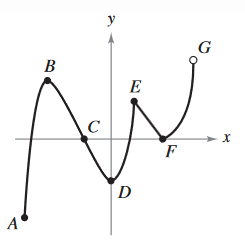
\includegraphics{54.png}
\begin{enumerate}[A:]
    \item Absolute minimum
    \item Relative maximum
    \item Neither
    \item Relative minimum
    \item Relative maximum
    \item Relative minimum
    \item Neither
\end{enumerate}

\section{Graph a function on the interval [-2, 5] having the given characteristics}
56. Relative minimum at $x=-1$, critical number (but no extremum) at $x=0$, absolute maximum at $x=2$, absolute minimum at $x=5$\\
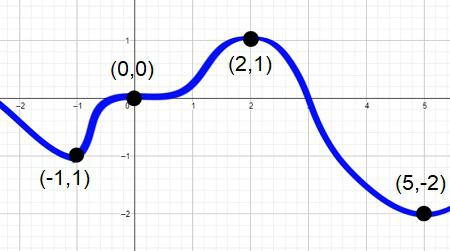
\includegraphics{56.jpeg}

\section{Determine from the graph whether $f$ has a minimum in the open interval $(a, b)$}
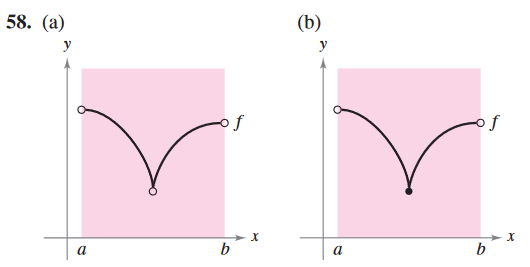
\includegraphics{58.png}
\begin{enumerate}[(a)]
    \item No
    \item Yes 
\end{enumerate}

\vspace{1cm}
\noindent
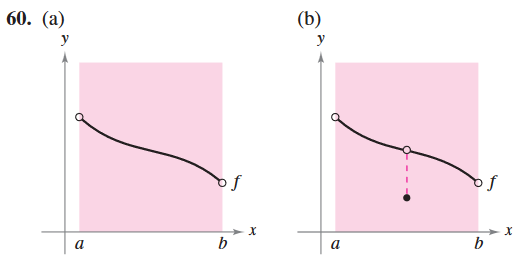
\includegraphics{60.png}
\begin{enumerate}[(a)]
    \item No
    \item Yes 
\end{enumerate}

\section{Determine whether the statement is true or false. If it is false, explain why or give an example that shows it is false.}
\noindent
65. The maximum of a function that is continuous on a closed interval can occur at two different values in the interval.\\
\\
\indent True

\vspace{1cm}
\noindent
66. If a function is continuous on a closed interval, then it must have a minimum on the interval.\\
\\
\indent True

\vspace{1cm}
\noindent
67. If $x=c$ is a critical number of the function $f$, then it is also a critical number of the function $g(x)=f(x)+k$, where $k$ is a constant.\\
\\
\indent True

\vspace{1cm}
\noindent
68. If $x=c$ is a critical number of the function $f$, then it is also a critical number of the function $g(x)=f(x-k)$, where $k$ is a constant.\\
\\
\indent False. $x=0$ is a critical number of $f(x)=x^2$. If $g(x)=f(x-k)=(x-k)^2$ then $x=k$ is a critical number of $g$.
\end{document}
